\documentclass[12pt, a4paper]{article}

% --- Font and Language Setup (Requires XeLaTeX compiler) ---
\usepackage[utf8]{inputenc}
\usepackage[T1]{fontenc}
\usepackage{carlito}
\renewcommand{\familydefault}{\sfdefault}

% --- Packages ---
\usepackage{geometry}
\geometry{top=2.5cm, bottom=2.5cm, left=2.5cm, right=2.5cm} % Standard academic margins
\usepackage{graphicx}
\usepackage{titlesec}
\usepackage[hidelinks]{hyperref}
\usepackage{xcolor}
\usepackage{listings}

% --- Python Code Formatting Setup ---
\definecolor{codegreen}{rgb}{0,0.6,0}
\definecolor{codegray}{rgb}{0.5,0.5,0.5}
\definecolor{codepurple}{rgb}{0.58,0,0.82}
\definecolor{backcolour}{rgb}{0.95,0.95,0.92}

\lstdefinestyle{mystyle}{
    backgroundcolor=\color{backcolour},   
    commentstyle=\color{codegreen},
    keywordstyle=\color{magenta},
    numberstyle=\tiny\color{codegray},
    stringstyle=\color{codepurple},
    basicstyle=\ttfamily\footnotesize,
    breakatwhitespace=false,         
    breaklines=true,                 
    captionpos=b,                    
    keepspaces=true,                 
    numbers=left,                    
    numbersep=5pt,                  
    showspaces=false,                
    showstringspaces=false,
    showtabs=false,                  
    tabsize=2
}
\lstset{style=mystyle}
\renewcommand{\lstlistingname}{Code Snippet}

% --- Document Info ---
\title{
    \Large \textbf{ITNPAI3: AI for NLP} \\
    \vspace{0.5cm}
    \LARGE \textbf{Deep Learning for Sentiment Analysis} \\
    \vspace{0.25cm}
    \large A Comparative Evaluation of Recurrent (BiLSTM) and Attention-Based (DistilBERT) Architectures
}
\author{Student ID: 3539054}
\date{April, 2026}

\begin{document}

\maketitle

\section{Data Preprocessing}

\quad Neural networks thrive on raw context, unlike statistical models that aggressively strip away grammar. To prevent damaging the structural and emotional meaning of the text, preprocessing was mostly limited to clearing out noise. To prepare the data without destroying its emotional context, the preprocessing pipeline focused on smart, targeted reduction:

\begin{itemize}
    \item \textbf{Standardising the Baseline:} The dataset used backticks in place of apostrophes, so this was fixed. URLs and mentions were swapped for placeholder tokens, reducing clutter while preserving sentence length.

    \item \textbf{Capturing the Emotion:} Emojis, heavy punctuation, and masked profanity were explicitly mapped to text tags. Words in all-caps were flagged before the entire dataset was lowercased, ensuring the neural network mathematically registers emotional spikes.

    \item \textbf{Preserving Grammar:} Most punctuation was stripped, but apostrophes were strictly kept to maintain contractions and negations. This allows the models to organically understand flipped sentiments without requiring manual coding.
\end{itemize}

\begin{table}[h!]
    \centering
    \renewcommand{\arraystretch}{1.5}
    \begin{tabular}{|p{0.45\textwidth}|p{0.45\textwidth}|}
        \hline
        \textbf{Raw Tweet} & \textbf{Preprocessed Tweet} \\ \hline
        
        Just updated \#Tweetie and open in browser is still broken. & just updated hashtag tweetie and open in browser is still broken \\ \hline
        
        A thursday. Is that REALLY necessary ? Have u ever heard of school and horrible mums & a thursday is that allcaps really necessary questionmark have u ever heard of school and horrible mums \\ \hline
    \end{tabular}
    \caption{Examples of preprocessing transformations.}
    \label{tab:preprocessing_examples}
\end{table}

\newpage

\noindent\begin{minipage}{\textwidth}
\begin{lstlisting}[language=Python, caption=Implementation of noise reduction and explicit emotional tokenisation.]
# Change backticks to standard apostrophes
text = text.replace("`", "'")

# Convert standalone '@' to 'at' (e.g., "meet me @ 8")
text = re.sub(r'(?:\s|^)@(?:\s|$)', ' at ', text)

# Replace mentions and URLs with structural tokens
text = re.sub(r"http\S+|www\S+|https\S+", ' urltoken ', text)
text = re.sub(r'\@\w+', ' usertoken ', text)

# Translate emoticons (<3 -> love)
# Replace spaces in the description with underscores
for emot_char, emot_desc in EMOTICONS_EMO.items():
    if emot_char in text:
        tokenized_desc = "_".join(emot_desc.replace(",", "").split())
        text = text.replace(emot_char, f" {tokenized_desc} ")

# Translate emojis
text = emoji.demojize(text, delimiters=(" ", " "))

# Tag hashtags (prefix with 'hashtag')
text = re.sub(r'#(\w+)', r' hashtag \1 ', text)
\end{lstlisting}
\end{minipage}

\vspace{0.5cm}

\section{Feature Representation}

\quad The \textbf{BiLSTM} model used a \textbf{word-level} tokenisation strategy, capping the vocabulary at 20,000 words. While this works for formal writing, it fails on Twitter, where slang and intentional misspellings (like "thanx") dominate. Any word outside that 20,000 word limit is replaced by a blank \textit{<OOV>} (Out-of-Vocabulary) token. This is a severe limitation as it actively erases rare but highly emotional words, blinding the network to critical sentiment signals before processing even begins.

\vspace{0.5cm}

To overcome the limitations of fixed vocabularies, \textbf{DistilBERT} utilises a \texttt{WordPiece} \textbf{subword} tokenisation strategy. Instead of discarding unknown words, it breaks down rare slang and misspellings into smaller, recognisable chunks (e.g., the slang 'allat' becomes 'all' \& 'at'). This approach virtually eliminates the Out-of-Vocabulary \texttt{(OOV)} problem. By breaking informal text into its core building blocks, it maximises coverage and provides a significantly richer foundation for the neural network.

\vspace{0.5cm}

Beyond handling rare words, the core difference between these models is contextual awareness. The \texttt{BiLSTM} relies on static definitions, meaning a word always has the exact same mathematical value regardless of how it is used. However, human emotion is deeply contextual. For example, the word "sick" can mean physical illness (negative) or extreme approval (positive slang), depending entirely on the surrounding sentence.

\vspace{0.5cm}

\texttt{DistilBERT} solves the static-word problem through contextual awareness. Instead of assigning a fixed definition, it processes the entire tweet simultaneously, dynamically adjusting the meaning of each word based on its surroundings. By mapping the fluid nature of human emotion rather than analysing vocabulary in rigid isolation, \texttt{DistilBERT} outperforms traditional word-level models.

\vspace{0.5cm}

\section{Model Training \& Evaluation}

\quad After training, \texttt{BiLSTM} and \texttt{DistilBERT} were evaluated on the original test set and directly benchmarked against the previous best statistical model (Logistic Regression with TF-IDF). To ensure a rigorous comparison, weighted metrics were used. This prevents the models from artificially inflating their accuracy by simply guessing the most common sentiment class.

\begin{table}[h!]
    \centering
    \renewcommand{\arraystretch}{1.5}
    \begin{tabular}{|l|c|c|c|c|}
        \hline
        \textbf{Model \& Representation} & \textbf{Accuracy} & \textbf{Precision} & \textbf{Recall} & \textbf{F1-Score} \\ \hline
        Logistic Regression (TF-IDF, C=10.0) & 0.692 & 0.697 & 0.692 & 0.694 \\ \hline
        BiLSTM (Word-Level) & 0.713 & 0.714 & 0.713 & 0.713 \\ \hline
        \textbf{DistilBERT (Subword)} & \textbf{0.786} & \textbf{0.791} & \textbf{0.786} & \textbf{0.786} \\ \hline
    \end{tabular}
    \caption{Performance metrics for each model and feature representation combinations.}
    \label{tab:model_performance}
\end{table}

While deep learning improved accuracy overall, the \texttt{BiLSTM} only managed a slight bump (from 69.2\% to 71.3\% accuracy). It successfully tracked word order but was severely crippled by its rigid vocabulary and zero pre-existing knowledge. Forced to learn English from scratch on a tiny dataset, the model quickly began memorising the data (\textbf{overfitting}) instead of truly understanding it, requiring intervention (regularisation and early stopping) to survive the training process.

\vspace{0.5cm}

In stark contrast, \texttt{DistilBERT} delivered a massive leap in performance, beating the baseline by nearly 8\% (78.6\% accuracy). This dominance comes from two core advantages. First, it uses \textbf{transfer learning}. Being pre-trained on massive datasets like Wikipedia, it already understood English grammar and nuance before seeing a single tweet. Second, its \textbf{self-attention} mechanism reads the entire tweet simultaneously. This allows it to instantly connect distant emotional cues without "forgetting" earlier words. Finally, its tightly grouped metrics prove the model is highly stable, classifying Positive, Negative, and Neutral text with equal confidence.

\vspace{0.5cm}

\section{Error Analysis}

\quad While \texttt{DistilBERT} is clearly the superior model, its errors highlight the current limits of neural models. A confusion matrix reveals that the model perfectly grasps extreme emotions: out of 3,534 tests, it almost never flipped a True Positive to a Negative, or vice versa. Instead, the vast majority of errors clustered around the Neutral category. The model frequently confused mildly emotional tweets with neutral ones. Because the line between "neutral" and "mildly emotional" is subjective even for humans, this Neutral bleed is an expected and natural limitation of the system.

\newpage

\begin{figure}[t]
    \centering
    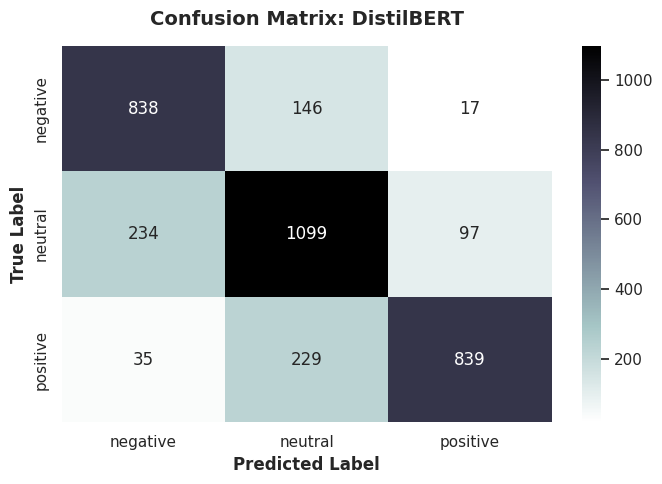
\includegraphics[width=0.8\textwidth]{confusion_matrix.png}
    \caption{Confusion Matrix for the \texttt{DistilBERT} (Subword) Model, demonstrating strong polar accuracy but notable bleeding around the "Neutral" class.}
    \label{fig:confusion_matrix}
\end{figure}

\noindent To understand why the model still struggled, a qualitative review of specific errors revealed some persistent blind spots (Table~\ref{tab:misclassifications}):

\begin{itemize}
    \item \textbf{Negation Handling:} While the model handles simple "nots," it fails on idioms. It sees "cant get much better" and over-indexes on the word "cant," misreading a peak positive statement as hesitant or neutral.

    \item \textbf{Mixed Sentiment:} When a tweet has mixed feelings, like being "so sad" but hoping things "might be better", the model anchors on the strongest keyword ("sad") instead of balancing the sentiment.

    \item \textbf{Sarcasm and Irony:} Sarcasm requires real-world logic. The model missed the insult in "pays more attention than my dead grandpa" because it doesn't biologically understand that a deceased person cannot pay attention.

    \item \textbf{Long-Range Dependencies:} The model flagged "cried so much" as pure sadness, failing to connect the tears to the talent show ("BGT") mentioned later. It missed the nuance that these were tears of joy or entertainment.

    \item \textbf{Named Entities:} Social media is saturated with pop-culture references that break standard linguistic rules. For instance, in the tweet "Terminator Salvation... by myself," the model fixates on the word "Salvation", which carries huge positive weight in general English, and incorrectly predicts a Positive sentiment. It fails to recognise that a highly emotional word is neutralised when it is simply part of a movie title.
\end{itemize}

\begin{table}[t]
    \centering
    \renewcommand{\arraystretch}{1.5}
    \begin{tabular}{|p{0.50\textwidth}|c|c|}
        \hline
        \textbf{Raw Tweet (Misclassified Examples)} & \textbf{True} & \textbf{Predicted} \\ \hline
        
        Hi all, just recovering from a party, looking forward to an exciting bank holiday around the diy shops...life cant get much better.surely & Positive & Neutral \\ \hline
        
        man im so sad school is ending but then again high school might be better :O & Neutral & Negative \\ \hline
        
        My dead grandpa pays more attention to me than you do & Negative & Neutral \\ \hline

        oh my god!!! i cried so much!!! watch this guys from BGT [urltoken] & Neutral & Negative \\ \hline
        
        Terminator Salvation... by myself & Neutral & Positive \\ \hline
    \end{tabular}
    \caption{Selected examples demonstrating neural model error patterns.}
    \label{tab:misclassifications}
\end{table}

\end{document}
